\subsection{System block diagram}
\label{sec:des-system}
The complete system connects page capture, handwriting interpretation and physical reproduction. The camera supplies an image to the ODROID N2+, while the gantry receives motion commands from the same computer. Between these interfaces, line images, recognised strings, writer probabilities and pen trajectories are kept as different representations. Figure~\ref{fig:des-hardware-system} shows the physical devices, supplies and signal paths; Figure~\ref{fig:des-processing-system} shows the software stages and the files passed between them. The text below explains how these two views relate to the project's functional units and how a page request reaches the gantry.


The hardware diagram distinguishes USB image data, GPIO control and switch feedback, motor power and mechanical coupling. The two A4988 drivers supply winding current to the X and Y motors; the ODROID supplies STEP and DIR signals rather than motor power through GPIO. Four switches provide axis-limit feedback and a fifth reports pen state. The pen motor has a separate transistor switching path. The Y drive's cross-shaft is a mechanical connection between the two belt sides, not an electrical signal. The server coordinates image acquisition, inference and job execution.


\begin{figure}[!htbp]\centering
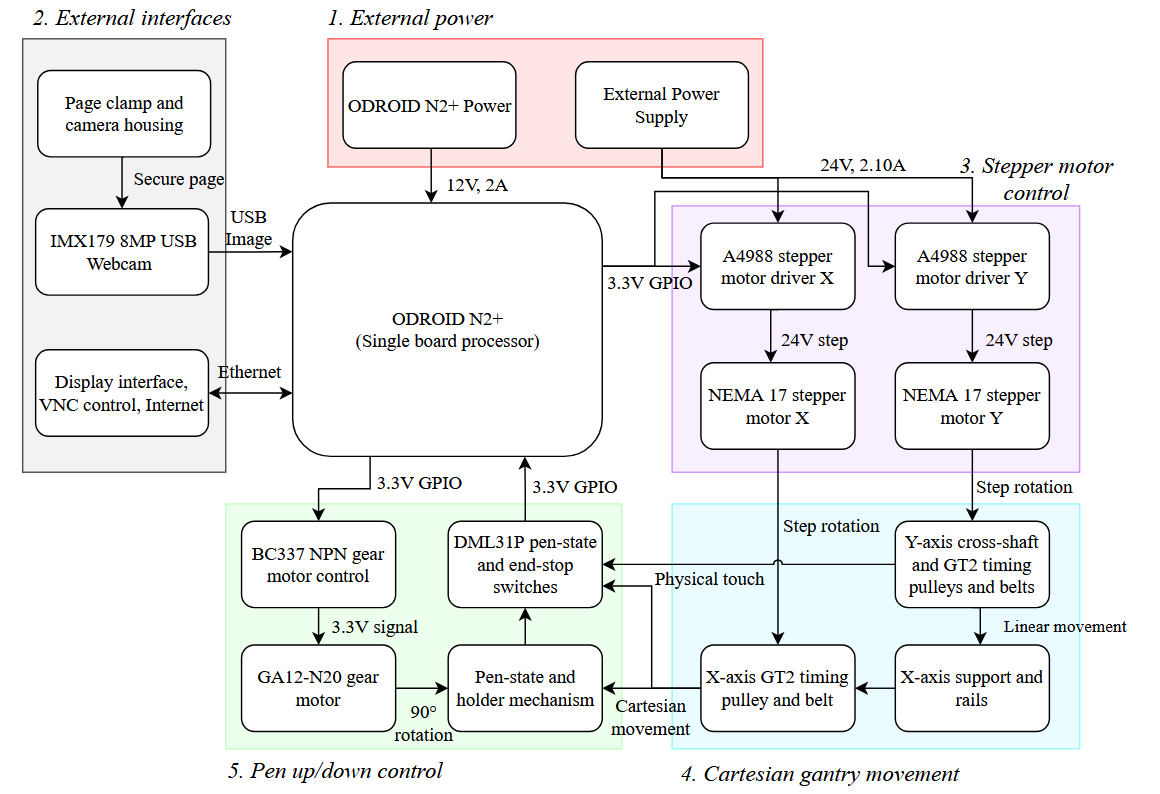
\includegraphics[width=0.96\linewidth]{Evidence/user_hardware_diagram_input.png}
\caption{Hardware system block diagram supplied by the author. The detailed controller pins, signal levels and power connections are listed in Table~\ref{tab:des-pin-map}.}
\label{fig:des-hardware-system}
\end{figure}

\begin{figure}[!htbp]\centering
\designasset{design-software-block-diagram.pdf}{0.96}{Three lanes for off-device preparation, ODROID page reading and ODROID writing. Show model training and transcript-guided glyph extraction; photographed page through conditioning, segmentation, reader and stroke-normalised writer vote; selected text/profile through best-of-N synthesis, trajectory and a G-code file boundary to the gantry interpreter. Draw model weights, line caches, profiles and job files as stored data. Include functional-unit identifiers on major blocks and a legend for processing, data, network and hardware-boundary links. Keep labels at least 8 pt at final size.}
\caption{Software block diagram showing preparation, page reading and handwriting generation.}
\label{fig:des-processing-system}
\end{figure}

\noindent\begin{minipage}{\linewidth}
The software diagram separates preparation, page reading and writing into three lanes. In preparation, labelled lines and known transcripts feed model training and transcript-guided glyph extraction; model weights, line caches and writer profiles are stored for later use. In page reading, conditioning and line segmentation precede the reader and stroke-normalised writer classifier, whose per-line outputs are combined into a page report. In writing, new text and a selected stored profile feed glyph layout and candidate scoring, then trajectory generation and a G-code file. The G-code file is the software-to-hardware boundary: the generator expresses geometry and pen state, while the gantry interpreter maps those commands to motor and pen signals. Training is identified as off-device; the request-time processing and motion stages are identified with the ODROID. The feedback from reader and writer scoring to candidate selection represents the implemented best-of-N search, not an independent measure of physical handwriting quality.
\end{minipage}

Recognition and reproduction share models, but they do not perform the same operation. Recognition estimates unknown text from an image. Glyph extraction uses text that is already known to estimate where its characters occur. Reproduction arranges the extracted pen paths into new text and uses the reader and writer classifier to select among candidate renderings. Keeping these roles separate is important: a candidate-selection score indicates how a model judges the generated image, whereas an independently assessed physical page establishes what the complete machine actually reproduced.

The final design reads complete lines rather than requiring isolated letters at FU 2.2. Character boundaries are instead recovered with known transcripts during profile construction. This avoids committing to uncertain cuts before recognising connected handwriting.

The proposal's functional units remain identifiable in this architecture. Camera acquisition and request handling implement FU~1; conditioning and line preparation implement FU~2.1--2.2; the two trained networks implement classification FU~2.3. Offline weight training corresponds to FU~2.4, while glyph extraction, profile storage and glyph retrieval implement FU~2.5--2.7. Trajectory conversion and the motion interpreter implement FU~2.8, followed by the axis drives, pen holder and lift in FU~3.1--3.4. Training and profile preparation produce stored artefacts before request-time recognition or writing; they are not repeated for each page.

The system-level distinction is also a practical commissioning boundary. G-code describes motion in millimetres and pen state without requiring the synthesiser to know GPIO pin assignments. Conversely, the motion interpreter can execute a geometric test file without loading handwriting models. A photographed page is therefore transformed into recognised text and a writer estimate through the read path; a separate writing request selects text and a stored writer profile, creates a trajectory and G-code, and sends that file to the interpreter. Keeping those requests distinct avoids implying that classifying a page alone causes the machine to reproduce it, while allowing faults to be located in image processing, trajectory generation or physical execution.
\FloatBarrier
